\chapter{Enthalpies of Reaction}\label{ch:b2:reaction-enthalpy}

A camping-gas cartridge screwed under a small burner: a few grams of
butane bring a litre of water to the boil in minutes, and the blue flame
under the pan is far hotter than the boiling water. How much heat does a
reaction release, how much of it reaches the pan, and how hot can the
flame get? None of these questions needs a burner to be answered: tables
of a few numbers per substance, measured once and for all, give the heat
of every reaction that can be written with those substances, at any
temperature. This chapter builds that bookkeeping. It applies the first
law of thermodynamics, known from physics, to a system whose composition
changes, defines the enthalpy of a reaction as a partial derivative, and
shows how to compute it from formation enthalpies, from bond enthalpies and
along cycles, how it changes with temperature, and what it says about
flames and calorimeters.

\begin{recall}
From physics: the first law $\Delta U = W + Q$; the enthalpy $H = U + pV$,
a state function; at constant external pressure, between two states at
that pressure, the heat received is $Q_p = \Delta H$; the heat capacity at
constant pressure $C_p = (\partial H/\partial T)_p$; the enthalpy of a
perfect gas depends on $T$ alone. The Year 1 volume described a reacting
system by its extent $\xi$ and the stoichiometric numbers $\nu_i$ of
$0 = \sum_i\nu_i\mathrm A_i$, and fixed the standard state of each species
at $p^\circ = \qty{1}{bar}$. The school volume (grade 11) called a reaction
\omterm{def:b2:reaction-enthalpy:exothermic}{exothermic} when it releases heat and estimated combustion energies from
bond energies.
\end{recall}

\begin{omfigure}
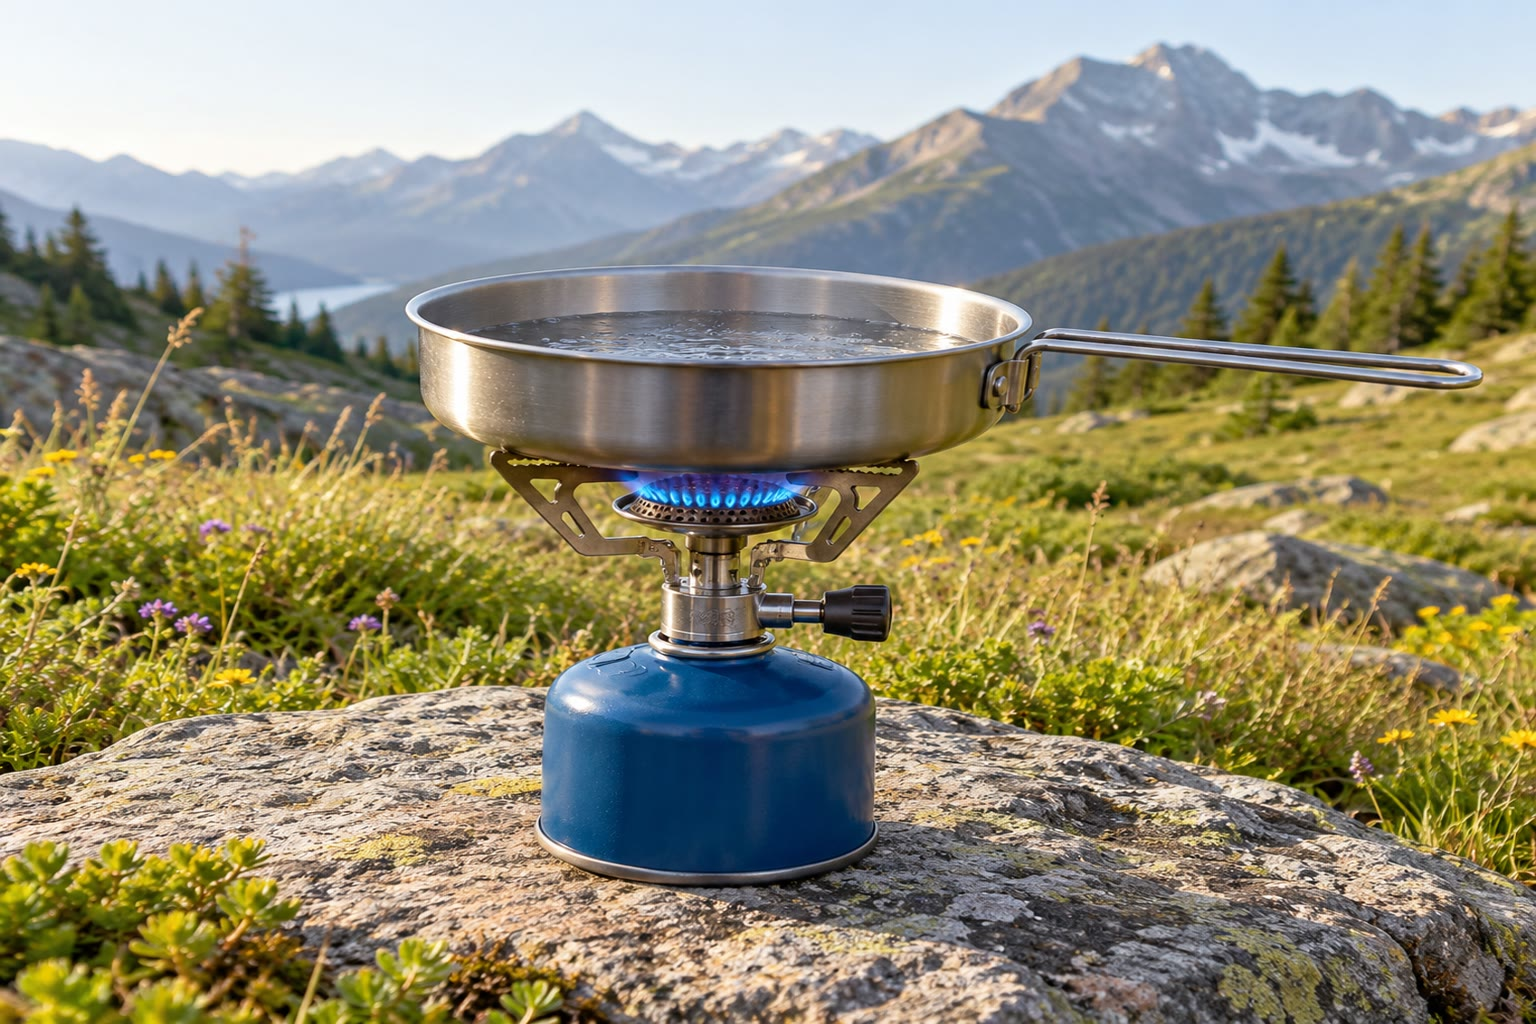
\includegraphics[width=0.6\linewidth]{images/book3/ai/b2-01-camping-stove.jpg}

{\small A camping stove: butane from the cartridge burns in the air under
the pan. The heat released per mole of butane, the share that reaches the
water and the temperature of the flame are computed in this chapter's
weekend problem.}
\end{omfigure}

\section{Reaction quantities}

A closed system in which the single reaction $0 = \sum_i\nu_i\mathrm A_i$
takes place is described by its temperature, its pressure and its extent:
the amounts are $n_i = n_{i,0} + \nu_i\xi$. Every extensive state function
of the system, its enthalpy for instance, is then a function $H(T, p,
\xi)$, and its exact differential is
\[
  \dd H = \left(\frac{\partial H}{\partial T}\right)_{p,\xi}\dd T
        + \left(\frac{\partial H}{\partial p}\right)_{T,\xi}\dd p
        + \left(\frac{\partial H}{\partial \xi}\right)_{T,p}\dd\xi .
\]

\begin{definition}[Reaction quantity, reaction enthalpy]\label{def:b2:reaction-enthalpy:reaction-quantity}
For an extensive state function $X$ of a closed system in which the
reaction $0 = \sum_i\nu_i\mathrm A_i$ takes place, the \emph{reaction
quantity}\index{reaction quantity} is the partial derivative
\[
  \Delta_r X = \left(\frac{\partial X}{\partial \xi}\right)_{T,p} ,
\]
the change of $X$ per unit extent at fixed temperature and pressure, in
units of $X$ per mole. For $X = H$ it is the \emph{reaction
enthalpy}\index{reaction enthalpy} $\Delta_r H$, in \unit{kJ/mol}.
\end{definition}

\begin{remark}[A derivative, not a difference]\label{rem:b2:reaction-enthalpy:operator}
The symbol $\Delta_r$ is an operator: it applies to the state of the
system, which it leaves unchanged. Writing the reaction differently
(doubling its coefficients) doubles $\Delta_r H$, so a \omterm{def:b2:reaction-enthalpy:reaction-quantity}{reaction quantity} is
meaningless without its equation. When the partial molar enthalpies
$\bar H_i = (\partial H/\partial n_i)_{T,p,n_j}$ of the species are used
(\cref{ch:b2:chemical-potential}), $\Delta_r H = \sum_i\nu_i\bar H_i$, by
the chain rule applied to $n_i = n_{i,0} + \nu_i\xi$.
\end{remark}

\begin{proposition}[Heat received at constant temperature and pressure]\label{prop:b2:reaction-enthalpy:qp}
When the reaction advances from $\xi_1$ to $\xi_2$ in a system kept at
constant $T$ and $p$, the system receives the heat
\[
  Q_p = \int_{\xi_1}^{\xi_2}\Delta_r H\,\dd\xi = \Delta_r H\,(\xi_2 - \xi_1)
\]
when $\Delta_r H$ does not depend on $\xi$.
\end{proposition}

\begin{proof}
At constant $p$ (and, here, constant external pressure), the heat received
is the change of enthalpy, $Q_p = \Delta H$ (physics). At fixed $T$ and $p$
the differential of $H$ reduces to $\dd H = \Delta_r H\,\dd\xi$; integrating
from $\xi_1$ to $\xi_2$ gives the result.
\end{proof}

\begin{definition}[Exothermic, endothermic, athermic]\label{def:b2:reaction-enthalpy:exothermic}
A reaction is \emph{exothermic}\index{exothermic} in a given state if
$\Delta_r H < 0$: run forward at constant $T$ and $p$, it gives heat to the
surroundings. It is \emph{endothermic}\index{endothermic} if $\Delta_r H >
0$, and \emph{athermic}\index{athermic} if $\Delta_r H = 0$.
\end{definition}

The heat of a reaction does not, in general, depend on the composition:
for perfect gases and for pure solids and liquids, the enthalpy of each
species does not depend on what surrounds it, and $\Delta_r H$ is fixed
once $T$ is.

\begin{proposition}[Ideal systems]\label{prop:b2:reaction-enthalpy:ideal}
In a mixture of perfect gases with pure condensed phases, $\Delta_r H$
depends on the temperature alone, and equals the \omterm{def:b2:reaction-enthalpy:standard-reaction-enthalpy}{standard reaction
enthalpy} $\Delta_r H^\circ(T)$ defined below. For solutes in dilute
solution the equality holds to a good approximation.
\end{proposition}

\begin{proof}
In a perfect-gas mixture each gas behaves as if alone, with an enthalpy
$n_iH_{m,i}(T)$ that does not depend on $p$ (physics: the enthalpy of a
perfect gas depends on $T$ only). A pure solid or liquid has $H = n_iH_{m,i}(T,
p)$, and $(\partial H_m/\partial p)_T = V_m(1 - \alpha T)$ is a few
\unit{J/(mol.bar)} for a condensed phase, negligible against reaction
enthalpies of tens of \unit{kJ/mol}. So $H = \sum_in_iH_{m,i}(T)$, whose
derivative with respect to $\xi$ is $\sum_i\nu_iH_{m,i}(T)$: it depends on
$T$ alone, and its value is the one computed with every species in its
standard state.
\end{proof}

\section{Standard reaction enthalpies and Hess's law}

\begin{definition}[Standard reaction quantity]\label{def:b2:reaction-enthalpy:standard-reaction-enthalpy}
The \emph{standard reaction quantity}\index{standard reaction quantity}
$\Delta_r X^\circ(T) = \sum_i\nu_iX_{m,i}^\circ(T)$ is the \omterm{def:b2:reaction-enthalpy:reaction-quantity}{reaction quantity}
computed with every species in its standard state at temperature $T$, the
$X_{m,i}^\circ$ being the standard molar values. For $X = H$ it is the
\emph{standard reaction enthalpy}\index{standard reaction enthalpy}
$\Delta_r H^\circ(T)$; it depends on $T$ only.
\end{definition}

Only differences of enthalpy are measurable, so a reference is chosen once
and for all, as the hydrogen electrode was chosen for potentials.

\begin{definition}[Standard reference state, standard enthalpy of formation]\label{def:b2:reaction-enthalpy:formation}
The \emph{standard reference state}\index{standard reference state} of an
element at temperature $T$ is its most stable form at $T$ under $p^\circ$:
\ce{H2}, \ce{O2}, \ce{N2} and \ce{Cl2} as perfect gases, carbon as
graphite, sodium as the metal, bromine as the liquid (at \qty{298}{K}).
The \emph{standard enthalpy of formation}\index{standard enthalpy of formation}
$\Delta_f H^\circ$ of a compound is the \omterm{def:b2:reaction-enthalpy:standard-reaction-enthalpy}{standard reaction
enthalpy} of its formation reaction, the one that makes one mole of the
compound from its elements in their reference states. By construction,
$\Delta_f H^\circ = 0$ for an element in its reference state.
\end{definition}

\begin{example}[Formation reactions]\label{ex:b2:reaction-enthalpy:formation}
The formation reaction of water is \ce{H2(g) + 1/2O2(g) -> H2O(l)}, with
$\Delta_f H^\circ = \qty{-285.83}{kJ/mol}$ at \qty{298.15}{K}; that of
methane is \ce{C(s) + 2H2(g) -> CH4(g)}, $\Delta_f H^\circ =
\qty{-74.9}{kJ/mol}$; that of nitrogen monoxide, \ce{1/2N2(g) + 1/2O2(g) ->
NO(g)}, $\Delta_f H^\circ = \qty{+90.3}{kJ/mol}$: an \omterm{def:b2:reaction-enthalpy:exothermic}{endothermic} compound,
which the hot gases of an engine nevertheless make. The half coefficients
are not a problem: the formation reaction is a bookkeeping device, not a
mechanism.
% ledger: dfh:H2O-l, dfh:CH4_g, dfh:NO_g
\end{example}

\begin{theorem}[Hess's law]\label{thm:b2:reaction-enthalpy:hess}
If a reaction is the sum, with coefficients $\lambda_k$, of reactions $k$,
its \omterm{def:b2:reaction-enthalpy:standard-reaction-enthalpy}{standard reaction enthalpy} is the same combination of theirs:
$\Delta_r H^\circ = \sum_k\lambda_k\Delta_r H_k^\circ$
(\emph{Hess's law}\index{Hess's law}). In particular, a \omterm{def:b2:reaction-enthalpy:standard-reaction-enthalpy}{standard reaction enthalpy}
can be computed along any path of reactions that leads from the
reactants to the products.
\end{theorem}

\begin{proof}
Each $\Delta_r H_k^\circ = \sum_i\nu_{i,k}H_{m,i}^\circ$ is linear in the
stoichiometric numbers. If the reaction is $\sum_k\lambda_k$ times the
reactions $k$, its stoichiometric numbers are $\nu_i = \sum_k\lambda_k
\nu_{i,k}$, and $\Delta_r H^\circ = \sum_i\nu_iH_{m,i}^\circ = \sum_k\lambda_k
\sum_i\nu_{i,k}H_{m,i}^\circ$. Behind the algebra is the first law: $H$ is a
state function, so its change between the same initial and final states
does not depend on the path.
\end{proof}

\begin{proposition}[Reaction enthalpy from formation enthalpies]\label{prop:b2:reaction-enthalpy:formation-sum}
$\Delta_r H^\circ(T) = \sum_i\nu_i\,\Delta_f H_i^\circ(T)$.
\end{proposition}

\begin{proof}
Take the path that decomposes the reactants into their elements in their
reference states (the reverse of their formation reactions, with the
coefficients $-\nu_i > 0$), then forms the products from the same elements
(coefficients $\nu_i > 0$). The elements cancel because the equation is
balanced, and \omterm{thm:b2:reaction-enthalpy:hess}{Hess's law} adds the enthalpies.
\end{proof}

\begin{omfigure}
\begin{tikzpicture}[font=\small, >={Stealth}, y=0.0062cm]
  \draw[->] (0,-1000) -- (0,180) node[above] {$H^\circ$ (\unit{kJ/mol})};
  \foreach \y in {0,-200,-400,-600,-800,-1000} \draw (-0.08,\y) -- (0.08,\y) node[left=4pt] {$\y$};
  % levels
  \draw[very thick] (1.0,0) -- (4.6,0) node[right] {\ce{C(s) + 2H2(g) + 2O2(g)}};
  \draw[very thick, omDef] (1.0,-74.9) -- (4.6,-74.9);
  \node[right, omDef] at (4.6,-110) {\ce{CH4(g) + 2O2(g)}};
  \draw[very thick, omThm] (1.0,-965.2) -- (4.6,-965.2) node[right] {\ce{CO2(g) + 2H2O(l)}};
  % arrows
  \draw[->, omDef, thick] (1.6,0) -- (1.6,-74.9);
  \node[omDef, anchor=south west, font=\footnotesize] at (1.1,5) {$\Delta_f H^\circ(\ce{CH4}) = -74.9$};
  \draw[->, omThm, thick] (3.9,0) -- (3.9,-965.2);
  \node[right, omThm, align=left] at (3.95,-500) {$\Delta_f H^\circ(\ce{CO2})$\\ $+ 2\Delta_f H^\circ(\ce{H2O})$\\ $= -965.2$};
  \draw[->, thick] (2.75,-74.9) -- (2.75,-965.2);
  \node[left, align=right] at (2.7,-650) {$\Delta_r H^\circ$\\ $= -890.3$};
\end{tikzpicture}

{\small Enthalpy levels for the combustion of methane at \qty{298.15}{K}.
The elements in their reference states are the zero. Methane lies
\qty{74.9}{kJ/mol} below them, the products \qty{965.2}{kJ/mol} below:
the combustion enthalpy is the difference, \qty{-890.3}{kJ/mol}, whatever
the path actually followed by the flame.}
% ledger: dfh:CH4_g, dfh:CO2, dfh:H2O-l
\end{omfigure}

\begin{example}[Combustion of methane]\label{ex:b2:reaction-enthalpy:methane}
For \ce{CH4(g) + 2O2(g) -> CO2(g) + 2H2O(l)},
$\Delta_r H^\circ = -393.51 + 2(-285.83) - (-74.87) - 0 =
\qty{-890.3}{kJ/mol}$ at \qty{298.15}{K}. The value measured in a
calorimeter is \qty{-890.7}{kJ/mol}: the table and the flame agree within
the uncertainty of the data. If the water leaves as vapour
($\Delta_f H^\circ = \qty{-241.83}{kJ/mol}$), $\Delta_r H^\circ =
\qty{-802.3}{kJ/mol}$: the difference, \qty{88.0}{kJ}, is the enthalpy of
vaporisation of two moles of water, which a gas boiler recovers by
condensing its fumes.
% ledger: dfh:CO2, dfh:H2O-l, dfh:CH4_g, dch:CH4, dfh:H2O_g (computed in figdata/bachelor-2/thermo-data.py)
\end{example}

\begin{method}[A Hess cycle]\label{met:b2:reaction-enthalpy:hess-cycle}
To find the enthalpy of a reaction that cannot be measured directly:
\begin{enumerate}
  \item write the target reaction with its states;
  \item find reactions of known enthalpy (combustions, formations) whose
        combination, with coefficients $\lambda_k$, gives the target;
  \item check that every species not in the target cancels;
  \item add the enthalpies with the same coefficients.
\end{enumerate}
\end{method}

\begin{example}[Carbon to carbon monoxide]\label{ex:b2:reaction-enthalpy:co}
Burning carbon always makes some carbon dioxide, so the enthalpy of
\ce{C(s) + 1/2O2(g) -> CO(g)} is not measured directly. The two combustions
\ce{C(s) + O2(g) -> CO2(g)} ($\qty{-393.51}{kJ/mol}$) and \ce{CO(g) +
1/2O2(g) -> CO2(g)} ($\qty{-283.0}{kJ/mol}$, measured) are; the target is
the first minus the second: $\Delta_r H^\circ = -393.51 + 283.0 =
\qty{-110.5}{kJ/mol}$, the formation enthalpy of carbon monoxide.
% ledger: dfh:CO2, dfh:CO_g
\end{example}

\begin{history}[Germain Henri Hess]
\begin{minipage}[t]{0.2\linewidth}\vspace{0pt}
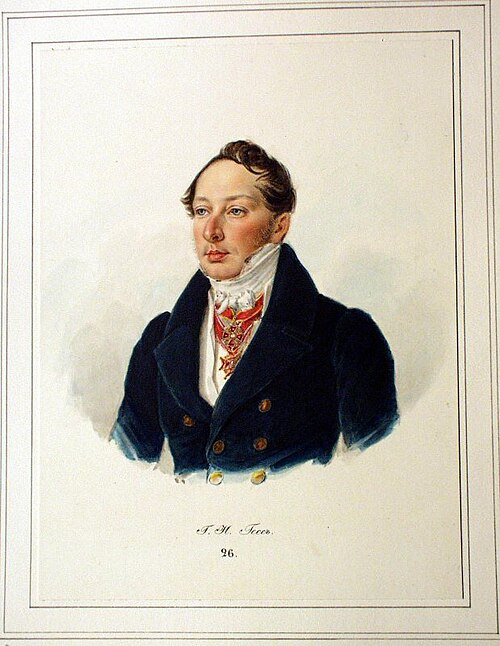
\includegraphics[width=\linewidth]{images/book3/hess.jpg}
\end{minipage}\hfill
\begin{minipage}[t]{0.76\linewidth}\vspace{0pt}
Germain Henri Hess (1802--1850), professor of chemistry in Saint
Petersburg, measured the heats released when sulfuric acid is diluted or
neutralised in several steps, and found in 1840 that the total did not
depend on the steps taken: the ``law of constant heat summation'', stated
before the first law of thermodynamics itself, which explains it.
(Portrait by I. I. Reimers, 1837--1838; CC BY-SA 4.0, Wikimedia Commons.)
\end{minipage}
\end{history}

\section{Computing reaction enthalpies}

\subsection*{From bond enthalpies}

When the formation enthalpy of a compound is missing, the energy of its
bonds gives an estimate, in the gas phase.

\begin{definition}[Bond dissociation enthalpy, mean bond enthalpy]\label{def:b2:reaction-enthalpy:bond-enthalpy}
The \emph{bond dissociation enthalpy}\index{bond dissociation enthalpy} of
a bond A--B in a gaseous molecule is the \omterm{def:b2:reaction-enthalpy:standard-reaction-enthalpy}{standard reaction enthalpy} of the
breaking of that bond into two gaseous fragments, \ce{AB(g) -> A(g) + B(g)}
for a diatomic molecule. When a molecule has $n$ equal bonds, its
\emph{mean bond enthalpy}\index{mean bond enthalpy} is the standard
enthalpy of its complete atomisation into gaseous atoms divided by $n$.
\end{definition}

The atomisation enthalpies are themselves formation enthalpies: those of
the gaseous atoms, minus that of the molecule. The table below is
computed in this way.

\begin{omfigure}
\begin{tabular}{lrl}
\hline
bond & enthalpy (\unit{kJ/mol}) & obtained from \\
\hline
H--H & 436 & \ce{H2}, dissociation \\
O=O & 498 & \ce{O2}, dissociation \\
N$\equiv$N & 945 & \ce{N2}, dissociation \\
Cl--Cl & 243 & \ce{Cl2}, dissociation \\
H--Cl & 432 & \ce{HCl}, dissociation \\
C--H & 416 & \ce{CH4}, mean of four \\
N--H & 391 & \ce{NH3}, mean of three \\
O--H & 464 & \ce{H2O}, mean of two \\
C=O & 804 & \ce{CO2}, mean of two \\
C--C & 330 & \ce{C2H6}, with C--H taken from methane \\
C=C & 589 & \ce{C2H4}, with C--H taken from methane \\
\hline
\end{tabular}

\smallskip
{\small Bond enthalpies at \qty{298.15}{K}, computed from the standard
enthalpies of formation of the gaseous atoms and molecules. The last two
lines show the limit of the method: a C--H bond of ethane is not exactly
one of methane, and the C--C value inherits the difference.}
% ledger: dfh:C_g, janaf:H, dfh:O_g, dfh:N_g, janaf:Cl, janaf:HCl, dfh:CH4_g, dfh:NH3_g, dfh:H2O_g, dfh:CO2, dfh:C2H6_g, dfh:C2H4_g (computed in figdata/bachelor-2/thermo-data.py)
\end{omfigure}

\begin{proposition}[Estimate from bond enthalpies]\label{prop:b2:reaction-enthalpy:bond-estimate}
For a reaction between gases,
\[
  \Delta_r H^\circ \approx \sum(\text{enthalpies of the bonds broken}) -
  \sum(\text{enthalpies of the bonds formed}).
\]
\end{proposition}

\begin{proof}
Follow the path that atomises every reactant (enthalpy: the bonds broken)
and then builds the products from the atoms (minus the bonds formed). \omterm{thm:b2:reaction-enthalpy:hess}{Hess's
law} makes the sum exact when each bond enthalpy is that of the bond in its
own molecule; replacing it by a mean value from another molecule is the
approximation.
\end{proof}

\begin{example}[Hydrogenation of ethene]\label{ex:b2:reaction-enthalpy:hydrogenation}
In \ce{C2H4(g) + H2(g) -> C2H6(g)}, one C=C and one H--H are broken and
replaced by one C--C and two C--H. With the table: $589 + 436 - 330 - 2
\times 416 = \qty{-137}{kJ/mol}$; from formation enthalpies the value is
\qty{-136.3}{kJ/mol}. The agreement is good here because the table's C--C
and C=C were obtained from these very molecules; for a molecule unlike
those of the table, an error of 10 to \qty{30}{kJ/mol} is common.
% ledger: dfh:C2H4_g, dfh:C2H6_g
\end{example}

\subsection*{Lattice enthalpies: the Born--Haber cycle}

\begin{definition}[Lattice enthalpy]\label{def:b2:reaction-enthalpy:lattice-enthalpy}
The \emph{lattice enthalpy}\index{lattice enthalpy} of an ionic crystal is
the \omterm{def:b2:reaction-enthalpy:standard-reaction-enthalpy}{standard reaction enthalpy} of its dissociation into gaseous ions: for
sodium chloride, \ce{NaCl(s) -> Na+(g) + Cl-(g)}. It is positive, and
measures the cohesion of the crystal.
\end{definition}

It cannot be measured directly, but a cycle through the elements gives it
from measurable quantities: the formation enthalpy of the crystal, the
atomisation of the elements, the ionisation energy of the metal and the
electron affinity of the non-metal (both defined in the Year 1 volume).

\begin{omfigure}
\begin{tikzpicture}[font=\small, >={Stealth}, y=0.0058cm]
  \def\lw{5.0}
  % levels (kJ/mol relative to Na(s) + 1/2 Cl2(g))
  \draw[thick] (0,0) -- (\lw,0) node[right] {\ce{Na(s) + 1/2Cl2(g)}};
  \draw[thick] (0,107.5) -- (\lw,107.5) node[right] {\ce{Na(g) + 1/2Cl2(g)}};
  \draw[thick] (0,228.8) -- (\lw,228.8) node[right] {\ce{Na(g) + Cl(g)}};
  \draw[thick] (0,724.6) -- (\lw,724.6) node[right] {\ce{Na+(g) + e- + Cl(g)}};
  \draw[thick] (0,376.1) -- (\lw,376.1) node[right] {\ce{Na+(g) + Cl-(g)}};
  \draw[thick] (0,-411.1) -- (\lw,-411.1) node[right] {\ce{NaCl(s)}};
  % the path through the elements, on the left
  \draw[->, omDef] (0.4,0) -- (0.4,107.5);
  \node[omDef, left, font=\footnotesize] at (0.35,53) {sublimation $107.5$};
  \draw[->, omDef] (0.4,107.5) -- (0.4,228.8);
  \node[omDef, left, font=\footnotesize] at (0.35,168) {$\tfrac12$ dissociation $121.3$};
  \draw[->, omDef] (0.4,228.8) -- (0.4,724.6);
  \node[omDef, left, font=\footnotesize] at (0.35,480) {ionisation of Na $495.8$};
  \draw[->, omThm] (1.4,724.6) -- (1.4,376.1);
  \node[omThm, right, font=\footnotesize] at (1.45,560) {electron attachment $-348.6$};
  \draw[->, omProp] (2.3,0) -- (2.3,-411.1);
  \node[omProp, left, font=\footnotesize] at (2.25,-205) {formation $-411.1$};
  % the lattice enthalpy, the only unknown
  \draw[->, thick] (3.6,-411.1) -- (3.6,376.1);
  \node[right, font=\footnotesize] at (3.65,-205) {lattice enthalpy $787$};
\end{tikzpicture}

{\small The Born--Haber cycle of sodium chloride at \qty{298}{K}
(\unit{kJ/mol}). Going up from the crystal to the gaseous ions by the
\omterm{def:b2:reaction-enthalpy:lattice-enthalpy}{lattice enthalpy}, or round by the elements, leads to the same level: the
\omterm{def:b2:reaction-enthalpy:lattice-enthalpy}{lattice enthalpy} is the only unknown of the cycle.}
% ledger: dfh:NaCl_cr, dfh:Na_g, janaf:Cl, ie:Na, ea:Cl
\end{omfigure}

\begin{method}[The Born--Haber cycle]\label{met:b2:reaction-enthalpy:born-haber}
\begin{enumerate}
  \item From the elements in their reference states, draw two paths: one
        to the crystal (formation), one to the gaseous ions (sublimation of
        the metal, atomisation of the non-metal, ionisation, electron
        attachment).
  \item Close the cycle with the \omterm{def:b2:reaction-enthalpy:lattice-enthalpy}{lattice enthalpy}, from the crystal up to
        the gaseous ions.
  \item Write that the sum of the enthalpies round the cycle is zero, and
        solve for the unknown. Ionisation energies and electron affinities
        are tabulated in eV per atom: multiply by $N_A e = \qty{96.485}{kJ/(mol.eV)}$.
\end{enumerate}
\end{method}

\begin{example}[Sodium chloride]\label{ex:b2:reaction-enthalpy:nacl}
$\Delta_{\text{lat}}H^\circ = 411.1 + 107.5 + 121.3 + 495.8 - 348.6 =
\qty{787}{kJ/mol}$. The ionisation energy and the electron affinity are
energies at \qty{0}{K}; their corrections to \qty{298}{K} ($+\tfrac52RT$
for each) cancel between the two steps. A crystal model with point charges
gives a similar value, which is why sodium chloride is called ionic.
% ledger: dfh:NaCl_cr, dfh:Na_g, janaf:Cl, ie:Na, ea:Cl (computed in figdata/bachelor-2/thermo-data.py)
\end{example}

\section{Reaction enthalpies and temperature}

Tables give $\Delta_f H^\circ$ at \qty{298.15}{K}. A reactor runs at
\qty{700}{K}, a flame at \qty{2000}{K}: how does $\Delta_r H^\circ$ change
with the temperature?

\begin{theorem}[Kirchhoff's law]\label{thm:b2:reaction-enthalpy:kirchhoff}
\[
  \frac{\dd\Delta_r H^\circ}{\dd T} = \Delta_r C_p^\circ =
  \sum_i\nu_i C_{p,m,i}^\circ ,
\]
so that $\Delta_r H^\circ(T_2) = \Delta_r H^\circ(T_1) + \int_{T_1}^{T_2}
\Delta_r C_p^\circ\,\dd T$ (\emph{Kirchhoff's law}\index{Kirchhoff's law}),
in the absence of a change of state between $T_1$ and $T_2$.
\end{theorem}

\begin{proof}
With every species in its standard state, $H^\circ(T, \xi) = \sum_in_i
H^\circ_{m,i}(T)$ is a function of two variables whose second partial
derivatives are continuous; by Schwarz's theorem they commute:
\[
  \frac{\dd\Delta_r H^\circ}{\dd T} = \frac{\partial}{\partial T}
  \frac{\partial H^\circ}{\partial\xi} = \frac{\partial}{\partial\xi}
  \frac{\partial H^\circ}{\partial T} = \frac{\partial}{\partial\xi}
  \sum_in_iC^\circ_{p,m,i} = \sum_i\nu_iC^\circ_{p,m,i}.
\]
Integrating between $T_1$ and $T_2$ gives the second form. A change of
state of a species inside the interval adds its enthalpy of transition,
with the stoichiometric number.
\end{proof}

\begin{example}[Ammonia synthesis when hot]\label{ex:b2:reaction-enthalpy:kirchhoff}
For \ce{N2(g) + 3H2(g) -> 2NH3(g)}, $\Delta_r H^\circ(298) =
\qty{-91.9}{kJ/mol}$ and, with the heat capacities at \qty{298}{K},
$\Delta_r C_p^\circ = 2(35.65) - 29.12 - 3(28.84) =
\qty{-44.3}{J/(K.mol)}$. Taken as constant, it gives $\Delta_r
H^\circ(700) = -91.9 - 0.0443 \times 402 = \qty{-109.7}{kJ/mol}$. The tables,
which follow the heat capacities as they grow with temperature, give
\qty{-105.2}{kJ/mol}: the constant-$C_p$ estimate is off by 4\,\%, a
fair price for a one-line computation. Over \qty{400}{K}, the \omterm{def:b2:reaction-enthalpy:reaction-quantity}{reaction
enthalpy} changes by about a seventh.
% ledger: dfh:NH3_g, cp:NH3_g.298, cp:N2_g.298, cp:H2_g.298, janafdfH:NH3.700 (computed in figdata/bachelor-2/thermo-data.py)
\end{example}

\section{Adiabatic reactions and calorimetry}

\subsection*{Flame temperature}

In a flame the reaction is fast and the heat has no time to leave: the
gases heat themselves.

\begin{definition}[Adiabatic flame temperature]\label{def:b2:reaction-enthalpy:flame-temperature}
The \emph{adiabatic flame temperature}\index{adiabatic flame temperature}
of a fuel is the temperature reached by the products of its complete
combustion when the reaction takes place at constant pressure, without
any exchange of heat, from reactants at \qty{298}{K}.
\end{definition}

\begin{proposition}[Computing a flame temperature]\label{prop:b2:reaction-enthalpy:flame}
If the reaction advances by $\xi$ from reactants at $T_0$ and the final
system has heat capacity $C_p(T)$, the final temperature $T_f$ satisfies
\[
  \xi\,\Delta_r H^\circ(T_0) + \int_{T_0}^{T_f}C_p(T)\,\dd T = 0 .
\]
\end{proposition}

\begin{proof}
Adiabatic and at constant pressure, the transformation has $\Delta H =
Q_p = 0$. As $H$ is a state function, any path between the same initial and
final states gives the same $\Delta H$. Take the path of
the figure below: first the reaction at $T_0$, with
$\Delta H_1 = \xi\Delta_r H^\circ(T_0)$ (\cref{prop:b2:reaction-enthalpy:qp},
with ideal behaviour); then the heating of the final system from $T_0$ to
$T_f$, $\Delta H_2 = \int C_p\,\dd T$. Their sum is zero.
\end{proof}

\begin{omfigure}
\begin{tikzpicture}[font=\small, >={Stealth}]
  \draw[->] (0,0) -- (6.2,0) node[right] {extent $\xi$};
  \draw[->] (0,0) -- (0,3.6) node[above] {temperature $T$};
  \fill (0.6,0.6) circle (2pt) node[below left] {reactants, $T_0$};
  \fill (5.2,0.6) circle (2pt) node[below] {products, $T_0$};
  \fill (5.2,3.0) circle (2pt) node[right] {products, $T_f$};
  \draw[->, thick, omDef] (0.7,0.6) -- (5.1,0.6);
  \node[omDef, above, font=\footnotesize] at (3.15,0.64) {$\Delta H_1 = \xi\,\Delta_r H^\circ(T_0) < 0$};
  \draw[->, thick, omThm] (5.2,0.7) -- (5.2,2.9);
  \node[omThm, right, align=left] at (5.25,1.8) {$\Delta H_2 = \int_{T_0}^{T_f} C_p\,\dd T$};
  \draw[->, thick, dashed] (0.75,0.75) -- (5.05,2.92);
  \node[above left, align=center] at (2.6,1.75) {real flame:\\ $\Delta H = 0$};
\end{tikzpicture}

{\small The adiabatic flame (dashed) and an equivalent path through two
steps: reaction at constant temperature, then heating of the products.
Since $H$ is a state function, the two enthalpy changes of the steps add
up to zero.}
\end{omfigure}

\begin{method}[Flame temperature]\label{met:b2:reaction-enthalpy:flame-temperature}
\begin{enumerate}
  \item Write the complete combustion of one mole of fuel; in air, add
        the nitrogen and argon that come with the oxygen (they are heated
        too); take the water as vapour.
  \item Compute $q = -\Delta_r H^\circ(T_0)$ per mole of fuel.
  \item Either take a constant heat capacity $C_p$ of the products:
        $T_f = T_0 + q/C_p$; or find $T_f$ such that the sum of the
        tabulated increments $n_i[H^\circ_{m,i}(T_f) - H^\circ_{m,i}(T_0)]$
        equals $q$, by interpolation.
\end{enumerate}
\end{method}

\begin{omfigure}
\begin{tikzpicture}
\begin{axis}[
  width=0.8\linewidth, height=6.2cm, xmin=300, xmax=3000, ymin=0, ymax=3200,
  axis x line=bottom, axis y line=left, xlabel={$T$ (K)},
  ylabel={$H(T) - H(\qty{298}{K})$ of the products (kJ)},
  xtick={500,1000,1500,2000,2500,3000},
  tick label style={font=\small}, label style={font=\small}, clip=false,
  legend style={font=\scriptsize, draw=none, at={(0.5,1.03)}, anchor=south}, legend columns=2]
\addplot[omDef, very thick] table[x=T, y=H] {figdata/out/bachelor-2-flame-temperature-butane.dat};
\addplot[omThm, very thick] table[x=T, y=H] {figdata/out/bachelor-2-flame-temperature-methane.dat};
\legend{1 mol butane in air, 1 mol methane in air}
\draw[omDef, dashed] (axis cs:300,2657.6) -- (axis cs:3000,2657.6);
\node[omDef, anchor=south east, font=\scriptsize] at (axis cs:2350,2657.6) {$-\Delta_r H^\circ = \qty{2657.6}{kJ}$};
\draw[omDef, dotted] (axis cs:2401,0) -- (axis cs:2401,2657.6);
\fill[omDef] (axis cs:2401,2657.6) circle (1.5pt);
\node[omDef, anchor=north west, font=\scriptsize] at (axis cs:2420,2620) {\qty{2401}{K}};
\draw[omThm, dashed] (axis cs:300,802.3) -- (axis cs:3000,802.3);
\node[omThm, anchor=south west, font=\scriptsize] at (axis cs:320,802.3) {$-\Delta_r H^\circ = \qty{802.3}{kJ}$};
\draw[omThm, dotted] (axis cs:2329,0) -- (axis cs:2329,802.3);
\fill[omThm] (axis cs:2329,802.3) circle (1.5pt);
\node[omThm, anchor=north west, font=\scriptsize] at (axis cs:2350,760) {\qty{2329}{K}};
\end{axis}
\end{tikzpicture}

{\small Enthalpy needed to heat the combustion products of one mole of
fuel (carbon dioxide, steam, and the nitrogen and argon of the air) from
\qty{298}{K}, from the tabulated enthalpies. Each curve meets the heat
released by its combustion at the \omterm{def:b2:reaction-enthalpy:flame-temperature}{adiabatic flame temperature}: about
\qty{2400}{K} for butane, \qty{2330}{K} for methane.}
% ledger: janafH:CO2.2400, janafH:H2O.2400, janafH:N2.2400, janafH:Ar.2400, air:N2, air:O2, air:Ar (computed in figdata/bachelor-2/flame-temperature.py)
\end{omfigure}

The computed temperatures are upper bounds. Above about \qty{2000}{K},
carbon dioxide and water begin to dissociate into carbon monoxide,
hydrogen, oxygen and radicals; these \omterm{def:b2:reaction-enthalpy:exothermic}{endothermic} reactions take back part
of the heat, and a real butane flame in air is noticeably cooler
than computed. In pure oxygen there is no nitrogen to heat and the flame is
much hotter, which is why welders burn ethyne with oxygen rather than with
air.

\subsection*{Calorimetry}

\begin{proposition}[Constant volume and constant pressure]\label{prop:b2:reaction-enthalpy:bomb}
In a closed steel vessel (a bomb calorimeter) the heat measured is $Q_V =
\Delta U$, and for perfect gases and condensed phases
\[
  \Delta_r H = \Delta_r U + \Delta\nu_{\text{gas}}\,RT ,
\]
where $\Delta\nu_{\text{gas}}$ is the sum of the stoichiometric numbers of
the gaseous species.
\end{proposition}

\begin{proof}
$H = U + pV$, and $\Delta_r H = \Delta_r U + \partial(pV)/\partial\xi$ at
fixed $T$. The $pV$ of the condensed phases is negligible, and for the
gases $pV = n_{\text{gas}}RT$ with $n_{\text{gas}} = n_{\text{gas},0} +
\Delta\nu_{\text{gas}}\xi$, whose derivative with respect to $\xi$ is
$\Delta\nu_{\text{gas}}RT$.
\end{proof}

\begin{omfigure}
\begin{tikzpicture}[font=\small, >={Stealth}, scale=1.0]
  % outer insulated jacket
  \draw[thick, fill=gray!8] (-2.6,-0.2) rectangle (2.6,4.4);
  \draw[thick, fill=white] (-2.3,0.1) rectangle (2.3,4.1);
  % water bath
  \fill[omDef!12] (-2.3,0.1) rectangle (2.3,3.4);
  \draw[omDef!60] (-2.3,3.4) -- (2.3,3.4);
  % bomb
  \draw[very thick, fill=gray!35] (-0.75,0.5) rectangle (0.75,2.6);
  \draw[very thick, fill=gray!55] (-0.9,2.6) rectangle (0.9,2.85);
  \draw[thick] (-0.3,1.0) -- (-0.3,1.9) (0.3,1.0) -- (0.3,1.9);
  \draw[thick, fill=orange!50] (-0.3,0.95) rectangle (0.3,1.05);
  \draw[red!70!black, thick, decorate, decoration={zigzag, amplitude=1pt, segment length=3pt}] (-0.3,1.9) -- (0.3,1.9);
  % wires
  \draw (-0.3,2.85) -- (-0.3,4.7) (0.3,2.85) -- (0.3,4.7);
  % stirrer and thermometer
  \draw[thick] (1.6,0.6) -- (1.6,4.7);
  \draw[thick, fill=gray!40] (1.35,0.55) rectangle (1.85,0.75);
  \pic[transform shape] at (-1.6,0.4) {thermometer};
  % labels
  \draw (-0.75,1.6) -- (-3.3,1.6) node[left] {steel bomb, \ce{O2} at 30 bar};
  \draw (0,1.0) -- (-3.3,0.6) node[left] {sample in its cup};
  \draw (0,1.9) -- (-3.3,2.6) node[left] {ignition wire};
  \draw (1.0,3.0) -- (3.3,3.0) node[right] {water bath};
  \draw (1.6,3.9) -- (3.3,4.3) node[right] {stirrer};
  \draw (-1.6,3.4) -- (-3.3,3.6) node[left] {thermometer};
  \draw (2.45,0.3) -- (3.3,0.5) node[right] {insulating jacket};
\end{tikzpicture}

{\small A bomb calorimeter. The sample burns at constant volume in
oxygen under pressure; the heat goes into the bomb and the stirred water,
whose temperature rise is read on the thermometer. The calorimeter's heat
capacity is found beforehand by burning a standard of known energy.}
\end{omfigure}

\begin{method}[Calorimetry]\label{met:b2:reaction-enthalpy:calorimetry}
\begin{enumerate}
  \item Calibrate: burn a mass of a standard of known energy of combustion
        (or pass a known electrical energy), read the temperature rise
        $\Delta T$, and deduce the heat capacity $C$ of the whole
        calorimeter (water and vessel, its ``water equivalent'').
  \item Burn the sample, read $\Delta T'$: the heat released is $C\,\Delta
        T'$, so $\Delta_r U = -C\Delta T'/\xi$ at constant volume.
  \item Correct to $\Delta_r H$ with $\Delta\nu_{\text{gas}}RT$; in an open
        (constant-pressure) calorimeter, $\Delta_r H = -C\Delta T'/\xi$
        directly.
\end{enumerate}
\end{method}

\begin{example}[A bomb measurement]\label{ex:b2:reaction-enthalpy:bomb}
For the combustion of butane with liquid water, $\Delta\nu_{\text{gas}} = 4
- 1 - 6.5 = -3.5$, so $\Delta_r U = \Delta_r H + 3.5RT = -2877.6 + 8.7 =
\qty{-2868.9}{kJ/mol}$: the correction is a few parts per thousand, larger
than the uncertainty of a good bomb measurement, so it is never omitted.
% ledger: dfh:C4H10_g, dfh:CO2, dfh:H2O-l (computed in figdata/bachelor-2/thermo-data.py)
\end{example}

\begin{history}[Calorimetric bombs, 1881]
\begin{minipage}[t]{0.2\linewidth}\vspace{0pt}
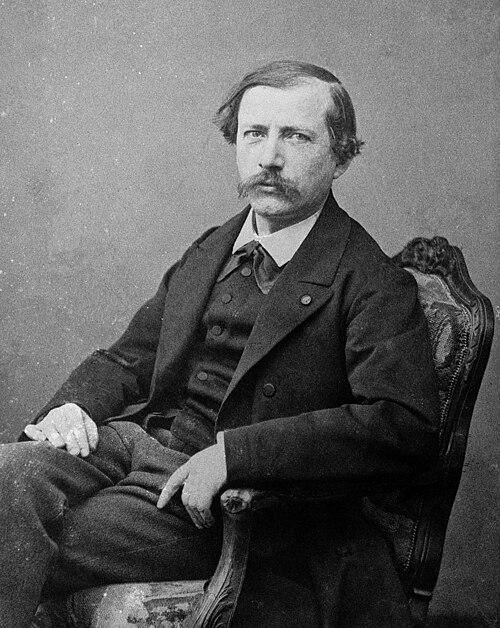
\includegraphics[width=\linewidth]{images/book3/berthelot.jpg}
\end{minipage}\hfill
\begin{minipage}[t]{0.76\linewidth}\vspace{0pt}
Marcellin Berthelot (1827--1907) burned organic compounds in compressed
oxygen inside a closed steel vessel lined with platinum, so that the
combustion was complete and nothing escaped: the calorimetric bomb, still
the instrument of record for heats of combustion. He also coined the words
\omterm{def:b2:reaction-enthalpy:exothermic}{exothermic} and \omterm{def:b2:reaction-enthalpy:exothermic}{endothermic}. (Photograph: public domain, Wikimedia
Commons.)
\end{minipage}
\end{history}

\section{Exercises}

\begin{exercise}[$\star$]\label{exo:b2:reaction-enthalpy:1}
Using the standard enthalpies of formation of the chapter, compute
$\Delta_r H^\circ$ at \qty{298}{K} of the combustion of propane,
\ce{C3H8(g) + 5O2(g) -> 3CO2(g) + 4H2O(l)}, given $\Delta_f
H^\circ(\ce{C3H8}, \text{g}) = \qty{-104.7}{kJ/mol}$. Is the reaction
\omterm{def:b2:reaction-enthalpy:exothermic}{exothermic}?
% ledger: dfh:C3H8_g
\end{exercise}

\begin{exercise}[$\star$]\label{exo:b2:reaction-enthalpy:2}
Compute the heat released by burning \qty{1.00}{kg} of methane (water
formed liquid) and \qty{1.00}{kg} of dihydrogen, \ce{H2(g) + 1/2O2(g) ->
H2O(l)}. Which fuel gives more heat per kilogram?
\end{exercise}

\begin{exercise}[$\star$]\label{exo:b2:reaction-enthalpy:3}
A bomb calorimeter gives $\Delta_r U = \qty{-3264}{kJ/mol}$ for liquid
benzene burning as \ce{C6H6(l) + 15/2O2(g) -> 6CO2(g) + 3H2O(l)} at
\qty{298}{K}. Compute $\Delta_r H$.
\end{exercise}

\begin{exercise}[$\star$]\label{exo:b2:reaction-enthalpy:4}
Given $\Delta_r H^\circ = \qty{-393.5}{kJ/mol}$ for \ce{C(s) + O2(g) ->
CO2(g)} and $\Delta_r H^\circ = \qty{-283.0}{kJ/mol}$ for \ce{CO(g) +
1/2O2(g) -> CO2(g)}, compute the enthalpy of \ce{CO2(g) + C(s) -> 2CO(g)},
the reaction that takes place in the hot coke of a blast furnace.
\end{exercise}

\begin{exercise}[$\star\star$]\label{exo:b2:reaction-enthalpy:5}
Estimate with the bond enthalpies of the chapter the enthalpy of
\ce{CH4(g) + Cl2(g) -> CH3Cl(g) + HCl(g)}, taking \qty{350}{kJ/mol} for
C--Cl. Then compute the same quantity from the formation enthalpies,
given $\Delta_f H^\circ(\ce{CH3Cl}, \text{g}) = \qty{-83.7}{kJ/mol}$, and
comment on the difference.
% ledger: dfh:CH3Cl_g
\end{exercise}

\begin{exercise}[$\star\star$]\label{exo:b2:reaction-enthalpy:6}
The standard enthalpy of vaporisation of water at \qty{298}{K} is
$\Delta_f H^\circ(\ce{H2O}, \text{g}) - \Delta_f H^\circ(\ce{H2O},
\text{l})$. Compute it. With $C_{p,m}^\circ = \qty{75.35}{J/(K.mol)}$ for
the liquid and \qty{33.59}{J/(K.mol)} for the vapour, both taken as
constant, estimate it at \qty{400}{K} (superheated water under pressure),
and compare with the tables, which give $\Delta_f H^\circ =
\qty{-282.59}{kJ/mol}$ for the liquid and \qty{-242.85}{kJ/mol} for the
vapour at \qty{400}{K}.
% ledger: cp:H2O_l.298, cp:H2O_g.298, janafdfH:H2O_l.400, janafdfH:H2O_g.400
\end{exercise}

\begin{exercise}[$\star\star$]\label{exo:b2:reaction-enthalpy:7}
Use a Born--Haber cycle to compute the \omterm{def:b2:reaction-enthalpy:lattice-enthalpy}{lattice enthalpy} of potassium
chloride from: $\Delta_f H^\circ(\ce{KCl}, \text{s}) = \qty{-436.7}{kJ/mol}$,
sublimation of potassium \qty{89.0}{kJ/mol}, ionisation energy of
potassium \qty{4.341}{eV}, $\Delta_f H^\circ(\ce{Cl}, \text{g}) =
\qty{121.3}{kJ/mol}$, electron affinity of chlorine \qty{3.613}{eV}. Why is
it smaller than that of sodium chloride?
% ledger: dfh:KCl_cr, dfh:K_g, ie:K, janaf:Cl, ea:Cl
\end{exercise}

\begin{exercise}[$\star\star$]\label{exo:b2:reaction-enthalpy:8}
A coffee-cup calorimeter is calibrated by passing \qty{2.00}{kJ} of
electrical energy, which raises its temperature by \qty{0.418}{K}. Then
\qty{50.0}{mL} of hydrochloric acid at \qty{1.00}{mol/L} is mixed in it
with \qty{50.0}{mL} of sodium hydroxide solution at \qty{1.10}{mol/L},
both at the same initial temperature: the temperature rises by
\qty{0.583}{K}. Compute the enthalpy of \ce{H3O+(aq) + OH-(aq) ->
2H2O(l)}.
\end{exercise}

\begin{exercise}[$\star\star$]\label{exo:b2:reaction-enthalpy:9}
Octane, a model of petrol, has $\Delta_f H^\circ(\text{l}) =
\qty{-250.3}{kJ/mol}$. Compute the enthalpy of its combustion (water
liquid), the heat released per kilogram, and the mass of carbon dioxide
emitted per megajoule. Compare with methane.
% ledger: dfh:C8H18
\end{exercise}

\begin{exercise}[$\star\star\star$]\label{exo:b2:reaction-enthalpy:10}
Compute the \omterm{def:b2:reaction-enthalpy:flame-temperature}{adiabatic flame temperature} of methane burning in the
stoichiometric amount of pure oxygen, with constant heat capacities (those
of the chapter at \qty{298}{K}: \ce{CO2} 37.13, \ce{H2O(g)}
\qty{33.59}{J/(K.mol)}). Compare with the result in air,
\qty{2780}{K} in the same approximation. Why is the true flame in oxygen
much colder than this computation says?
% ledger: cp:CO2_g.298, cp:H2O_g.298
\end{exercise}

\begin{exercise}[$\star\star\star$]\label{exo:b2:reaction-enthalpy:11}
The heat capacity of a gas is often written $C_{p,m}^\circ = a + bT$. For
the synthesis of ammonia, take $\Delta_r a = \qty{-60.5}{J/(K.mol)}$ and
$\Delta_r b = \qty{0.0540}{J/(K^2.mol)}$ (fitted to the tables between
\qty{300}{K} and \qty{800}{K}). Integrate \omterm{thm:b2:reaction-enthalpy:kirchhoff}{Kirchhoff's law} from
\qty{298}{K} to \qty{700}{K} and compare with the value in the tables,
\qty{-105.2}{kJ/mol}, and with the constant-$C_p$ estimate.
\end{exercise}

\begin{exercise}[$\star\star\star$]\label{exo:b2:reaction-enthalpy:12}
Nitrogen monoxide forms in engines by \ce{N2(g) + O2(g) -> 2NO(g)}.
Compute its \omterm{def:b2:reaction-enthalpy:standard-reaction-enthalpy}{standard reaction enthalpy} at \qty{298}{K}. Show that, if
$\Delta_r C_p^\circ$ is small, the reaction absorbs about the same heat at
\qty{2000}{K}; using the heat capacities of the tables at \qty{298}{K}
(\ce{NO} \qty{29.85}{J/(K.mol)}, \ce{N2} 29.12, \ce{O2}
\qty{29.38}{J/(K.mol)}), estimate the change between
\qty{298}{K} and \qty{2000}{K}. Explain why an \omterm{def:b2:reaction-enthalpy:exothermic}{endothermic} reaction can be
a problem precisely in the hottest flames.
% ledger: dfh:NO_g, cp:NO_g.298, cp:N2_g.298, cp:O2_g.298
\end{exercise}

\section{Problem: The Camping-Gas Cartridge}

\begin{problem}[{Weekend problem --- the energy of butane, a measurement in
a bomb calorimeter, the water heated in a pan, and the temperature of the
flame}]
\label{pb:b2:reaction-enthalpy:1}
A camping stove burns butane from a cartridge holding \qty{230}{g}.
Data at \qty{298}{K} ($\Delta_f H^\circ$ in \unit{kJ/mol}): \ce{C4H10(g)}
$-125.6$, \ce{CO2(g)} $-393.51$, \ce{H2O(l)} $-285.83$, \ce{H2O(g)}
$-241.83$. Molar masses: \ce{C4H10} \qty{58.12}{g/mol}, \ce{H2O}
\qty{18.02}{g/mol}. Heat capacity of liquid water
\qty{75.35}{J/(K.mol)}. Dry air: \qty{20.95}{\percent} \ce{O2},
\qty{78.08}{\percent} \ce{N2}, \qty{0.93}{\percent} \ce{Ar} by volume. $R = \qty{8.314}{J/(K.mol)}$.
% ledger: dfh:C4H10_g, dfh:CO2, dfh:H2O-l, dfh:H2O_g, cp:H2O_l.298, air:O2, air:N2, air:Ar

\medskip
\noindent\textbf{Part I --- The fuel.}
\begin{enumerate}
  \item Write the complete combustion of butane, water formed liquid,
        for one mole of butane.
  \item Compute its \omterm{def:b2:reaction-enthalpy:standard-reaction-enthalpy}{standard reaction enthalpy} at \qty{298}{K}.
  \item Compute it again with the water formed as vapour, and explain the
        difference.
  \item Compute the heat released per gram of butane in each case.
  \item Which of the two values describes a camping stove, whose water
        leaves the flame as vapour?
  \item What heat can the whole cartridge release on the stove?
\end{enumerate}

\medskip
\noindent\textbf{Part II --- A measurement.}
A sample of \qty{0.500}{g} of butane is burnt in a bomb calorimeter whose
heat capacity is \qty{10.00}{kJ/K}; the water formed condenses.
\begin{enumerate}[resume]
  \item What quantity does a bomb calorimeter measure, and why?
  \item Compute $\Delta\nu_{\text{gas}}$ of the reaction of question 1.
  \item Compute the expected $\Delta_r U$.
  \item Compute the expected temperature rise of the calorimeter.
  \item The rise read is \qty{2.461}{K}. Deduce the measured $\Delta_r U$
        and $\Delta_r H$, and the relative difference with the tables.
\end{enumerate}

\medskip
\noindent\textbf{Part III --- The pan.}
\begin{enumerate}[resume]
  \item Compute the heat needed to bring \qty{1.00}{L} of water
        (\qty{1.00}{kg}) from \qty{20}{\celsius} to \qty{100}{\celsius}.
  \item The stove does it with \qty{16.0}{g} of butane. Compute its
        efficiency (heat received by the water over heat released).
  \item Where does the rest of the heat go?
  \item How many litres of water can the whole cartridge bring to the boil
        at this efficiency?
\end{enumerate}

\medskip
\noindent\textbf{Part IV --- The flame.}
\begin{enumerate}[resume]
  \item Butane burns in the stoichiometric amount of air. Compute the
        amounts of dinitrogen and argon that come with the dioxygen needed
        by one mole of butane.
  \item List the amounts of the products, nitrogen and argon included.
  \item Explain, with a two-step path, why the heat released at
        \qty{298}{K} by the reaction (water as vapour) is entirely used to
        heat these gases.
  \item Using the heat capacities at \qty{298}{K}, \ce{CO2} 37.13,
        \ce{H2O(g)} 33.59, \ce{N2} 29.12, \ce{Ar} \qty{20.79}{J/(K.mol)},
        compute the heat capacity of the products.
  \item Deduce the flame temperature with constant heat capacities.
  \item The enthalpy increments of the tables give, for the products of one
        mole of butane, \qty{2515.7}{kJ} between \qty{298}{K} and
        \qty{2300}{K}, and \qty{2655.7}{kJ} between \qty{298}{K} and
        \qty{2400}{K}. Find the flame temperature by linear interpolation.
  \item Why is the first estimate too high?
  \item Why is the measured temperature of a butane flame lower still?
  \item State the \omterm{def:b2:reaction-enthalpy:flame-temperature}{adiabatic flame temperature} of butane in air.
\end{enumerate}
\end{problem}
